\documentclass[oneside]{book}
\usepackage[utf8]{inputenc}
\usepackage[outline]{contour}
\usepackage[dvipsnames]{xcolor}
\usepackage{enumitem}
\usepackage{amsmath}
\usepackage{amssymb}
\usepackage{amsfonts}
\usepackage[normalem]{ulem}
\usepackage{mathrsfs}  
\newtheorem{theorem}{Theorem}
\newtheorem{corollary}{Corollary}[theorem]
\newtheorem{lemma}[theorem]{Lemma}
\usepackage{tikz}

\usepackage{fullpage}

\AddToHook{shipout/background}{%
\put (0in,-\paperheight){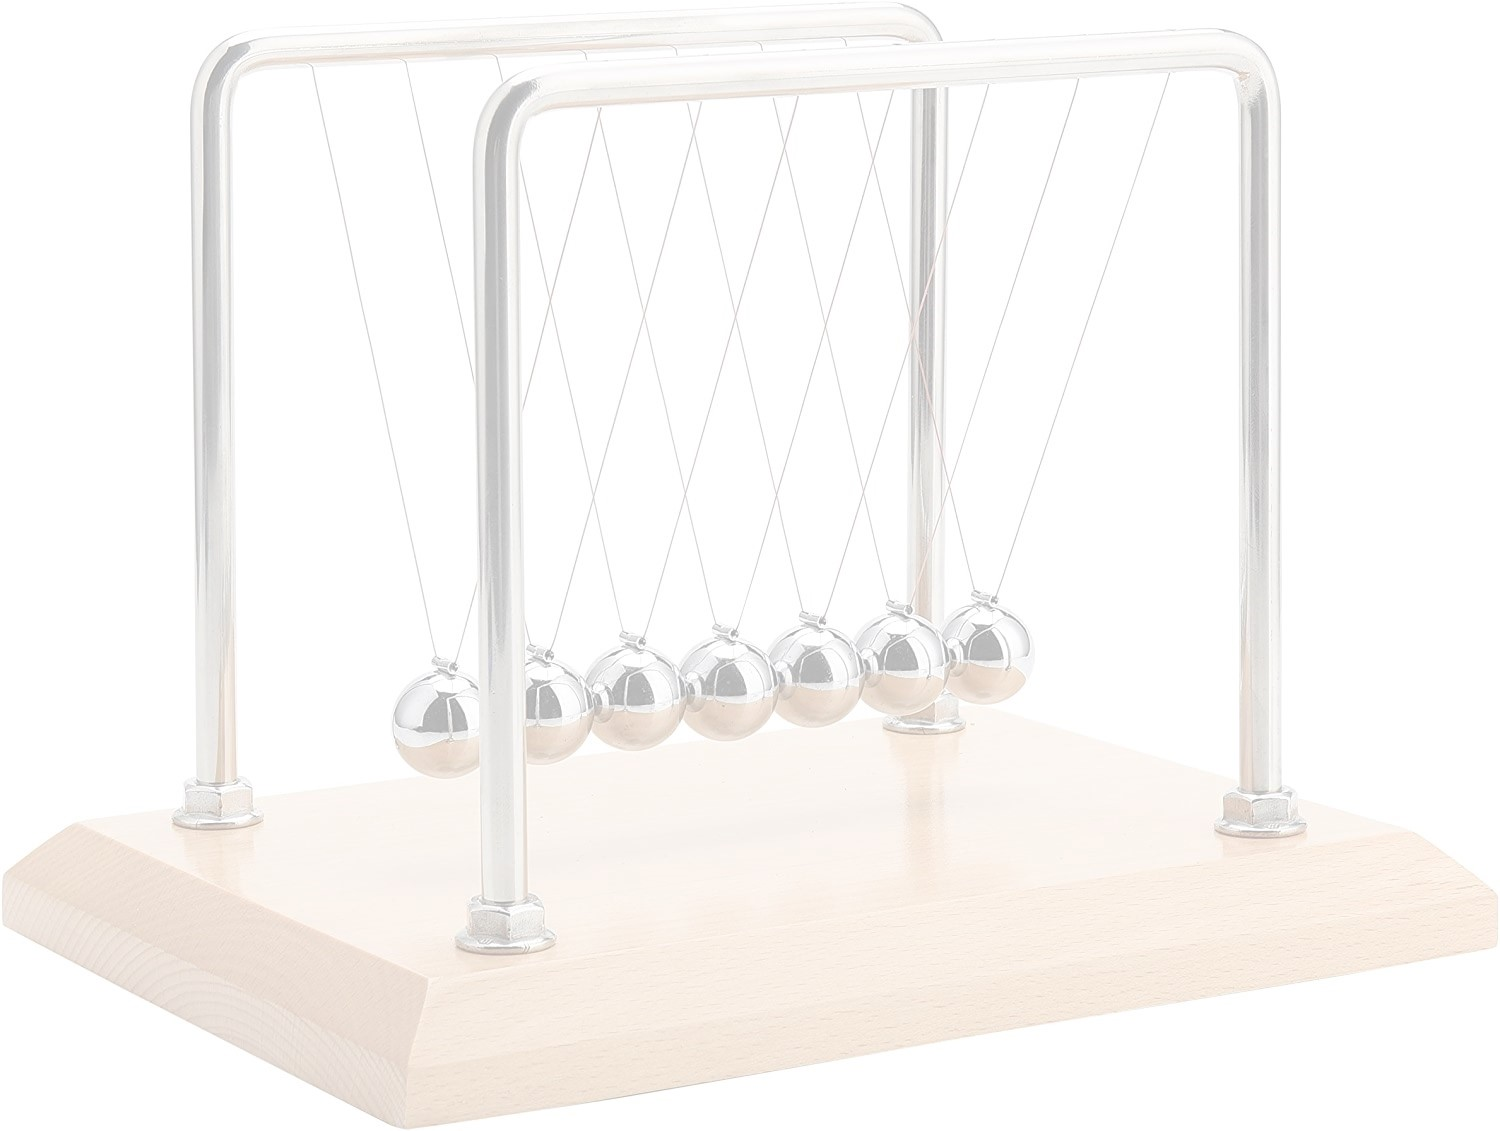
\includegraphics[width=\paperwidth,height=\paperheight]{Newton.jpg}}%
}
\usepackage{graphicx}
\graphicspath{ {./images/} }

\usepackage[pagestyles]{titlesec}
\titleformat{\chapter}[display]   
{\normalfont\huge\bfseries}{\chaptertitlename\ \thechapter}{20pt}{\Huge}   
\titlespacing*{\chapter}{0pt}{-50pt}{40pt}
\titleformat{\chapter}[display]{\normalfont\bfseries}{}{0pt}{\Huge}
\newpagestyle{mystyle}
{\sethead[\thepage][][\chaptertitle]{}{}{\thepage}}
\pagestyle{plain}
\setcounter{secnumdepth}{0}

\usepackage{geometry}
\geometry{
  bottom=15mm
}

\usepackage{hyperref}
\hypersetup{
    colorlinks=true,
    linkcolor=ProcessBlue!30,
    filecolor=magenta,      
    urlcolor=cyan,
    }

\begin{document}
\pagecolor{white}

  \begin{tikzpicture}[font=\sffamily,remember picture,overlay]
      \node[fill={rgb:pink,0.5;orange,1;yellow,0.5},anchor=north, minimum width=\paperwidth, minimum height=2cm] (names)
   at ([yshift=0cm]current page.north) {
    \begin{tabular}{c}
        \\
        \color{white} \contourlength{0.5pt}\contour{black}{\fontsize{24.88pt}{65pt}\selectfont Physics Paper 3 Notes}\\[2mm]
        \Large \color{white} \contourlength{0.5pt} \contour{black}{Grass}\\
        \\
    \end{tabular}
    };
\end{tikzpicture}

\footnotesize
\begingroup
\let\clearpage\relax
\vspace{1cm}
\chapter{Planning Exercise}
\mainmatter
\endgroup
\raggedright
\section{V-CID [1m]}
\subsection{Constant Variables}
E.g.:
\begin{enumerate}
    \item Material of the lens
    \item Distance \(y\) 
    \item Type of material of the glass block
    \item Length of nichrome wire
\end{enumerate}
\begin{itemize}[label=\(\square\)]
    \item At least \colorbox{Goldenrod}{one constant variable} (Not \colorbox{pink}{environmental variables}, must be \colorbox{green}{controllable})
\end{itemize}
\subsection{Independent Variable:}
E.g.:
\begin{enumerate}
    \item Focal length of the different lenses
    \item \(u\) (Object distance in \(cm\))
    \item Vertical height, \(h/cm\) 
\end{enumerate}
\subsection{Dependent Variable:}
\begin{enumerate}
    \item Image distance, \(x\) 
    \item \(v\) (Image distance in \(cm\))
    \item Time taken, \(T/s\) for the marble to roll the distance \(d\).
\end{enumerate}
\section{Steps:}
\subsection{mrc (Meaure, Record, Calculate)}
\begin{enumerate}
    \item \textbf{Set up the apparatus as shown in the diagram}\\
    \item[\vdots \vspace{1mm} ] (Describe how to collect the dependent variable)
    \item[\(n.\)] Calculate \uline{(whatever you need for graphing [E.g.: \(\frac{1}{T^2}\)] )}
    \item[\(n+1\).] \textbf{While keeping the key variables constant, repeat steps 2 to \(\mathbf{k}\) for a total of 6 sets of data for \uline{(independent variable)} and \uline{(dependent variable)}}  
\end{enumerate}
\begin{itemize}[label=\(\square\)]
    \item Copy words from the \colorbox{yellow}{short experiment instructions}. \colorbox{red}{DO NOT} change them into your own words.
\end{itemize}
\subsection{tgr (Tabulate, plot Graph, conclude Relationship)} 
\begin{enumerate}[label=\(n+\arabic*.\)]
    \setcounter{enumi}{1}
    \item Tabulate all the readings of \footnotesize \uline{(whatever you need for your graph + what you originally recorded)} \footnotesize
    \item Plot a graph of \uline{(variable for vertical axis)} against \uline{(variable for horizontal axis)}
    \item If the relationship is true, the graph should \uline{[E.g.: show a straight line with a positive gradient cutting through the origin]}
    \item To determine \uline{(constant in the equation given [E.g.: \(G\) in \(f=G ( \frac{x}{y} )\)] )}, calculate the gradient of the graph. \uline{(Add somemore stuff if somemore manipulation is needed to determine that constant)}. 
\end{enumerate}
\newpage
\chapter{Accuracy and other Notes}
\begin{itemize}[label=\(\square\)]
    \item Literally \textbf{everything 3 s.f.}
    \item Rmb to put the correct units in the answers.\\
    \scriptsize E.g.: \(t=x\,s\), \(E=x\,J\), \(c=x\,J/g^{\circ}C\), \(G=x\) (The gradient might not have any units attached) \footnotesize
    \item Careful of the table labels. \colorbox{red}{Do not} put units in your readings or write down the readings for the wrong units.
    \item \bigskip 
    \begin{tabular}{|c|c|c|c|c|c|}
        \hline 
        No. & Instrument & Smallest div & Uncertainty / Accuracy & No. of dp & Examples\\
        \hline
        1 & Ammeter & 0.02\(A\) & 0.01\(A\) & 2 & 0.20\(A\), 0.21\(A\)\\ 
        \hline
        2 & Electronic Balance & 0.01\(g\) & \(0.01g\) & 2 & \(121.10g\), \(121.01g\)\\
        \hline
        3 & Metre Rule & 0.1\(cm\) & \(0.1cm\) & 1 in \(cm\) & 12.0\(cm\), \(12.1cm\)\\
        \hline
        4 & Measuring Cylinder & 1\(cm^3\) & \(0.5cm^3\) & 1 & \(18.0cm^3\), \(18.5cm^3\)\\
        \hline
        5 & Spring Balance & 0.1\(N\) & 0.05\(N\) & 2 & \(3.65N\), \(3.70N\)\\
        \hline
        6 & Stopwatch & 0.01\(s\) & 0.01\(s\) & 2 & \(28.11s\)\\
        \hline
        7 & Thermometer & \(1\) \(^{\circ}C\) & \(0.5\) \(^{\circ}C\) & 1 & \(23.0\) \(^{\circ}C\), 23.5 \(^{\circ}C\)\\
        \hline
        8 & Voltmeter & \(0.1V\) & \(0.05V\) & 2 & \(1.50V\), \(1.55V\)\\
        \hline
    \end{tabular}
    \item Types of relationships / graphs
    \begin{enumerate}
        \item Directly Propertional -- Passes through the origin + Straight line (+/- gradient doesn't matter)
        \item Linearly related (either with +/- gradient) -- Doesn't cut origin + Straight line 
        \item Inversely Propertional -- Looks similar to \(\frac{1}{x}\). Well, by definition, it should follow a form of \(y=\frac{k}{x}\), where \(k\) is constant. 
    \end{enumerate}
\end{itemize}
\begingroup
\vspace{2.5cm}
\let\clearpage\relax
\chapter{Example Qns}
\endgroup

\section{Accuracy}
\begin{enumerate}
    \item Suggest \textbf{two} ways in which you assembled the apparatus to make the temperature readings accurate.
    \begin{itemize}[label=\(\circ\)]
        \item Ensure that the thermometer is clamped vertically to avoid parallex error.
        \item ENsure that the bulb of the thermometer is fully immersed in the oil.
        \item Ensure the resistors are fully immersed in the oil.
    \end{itemize}
    \item Explain two sources of error in the experimental procedure that cause the value of \(c_1\) to be different from the value of \(c_2\). \scriptsize [\(c_1\) and \(c_2\) are values for specific heat capacity calculated with 2 different ways] \footnotesize
    \begin{itemize}[label=\(\circ\)]
        \item Some thermal energy is lost ot the surroundings from the uncovered oil
        \item The current reading drops slightly during the experiement as the resistors and the oil gets hotter. \scriptsize (This was an observation when actually conducting the expt) \footnotesize
    \end{itemize}
    \item Suggest one reason why the actual length \(L\) of the resistance wire in the coil is different from the value calculated in \((h)(i)\) \scriptsize [theoretical calculation from equation given] \footnotesize. 
    \begin{itemize}[label=\(\circ\)]
        \item The wire on the metre rule cannot be fully straightened
        \item There is a section of resistance wire which is not coiled and also not on the metre rule
        \item Temperature of resistance wire rose while current was flowing. So, resistance was not constant, and hence, the voltage recorded was affected.
    \end{itemize}
    \item Identify any key sourcesof error and explain how the yaffect the accuracy of the readings. \scriptsize [Find refracted angle of a ray of light in glass block expt] \footnotesize
    \begin{itemize}[label=\(\circ\)]
        \item The holes made by the pins are rather large. This affects the accuracy in constructing the path of the incident and emergent rays.
        \item The glass block, with bevelled edges, makes it hard to replace the block on the exact position each time. Thus, the value of \(i\) and \(r\) may be inconsistent.
    \end{itemize} 
    \item State ONE key source of error in this experiement. \scriptsize [Resistance Experiment] \footnotesize\\
    \begin{itemize}[label=\(\circ\)]
        \item The temperature of the fixed resistor increases with time.
    \end{itemize}
    \item State \textbf{one} key source of error for this experiement.\\
    \begin{itemize}[label=\(\circ\)]
        \item The sharpness of the image is an estimation. This affects the accuracy of distance \(x\) measured. \scriptsize [Converging Lens Expy] \footnotesize
        \item The centre of the lens may not be accurate. This affects the accuracy of distances \(x\) and \(y\) measured.
    \end{itemize}
    \item  Explain whether your value for \(a\) in \textbf{(d)}
    supports the suggestion made by the student in \textbf{(e)}.\\
    \begin{itemize}[label=\(\circ\)]
        \item No. Suggestion in (e) does not take into account the energy lost due to friction.
    \end{itemize}
\end{enumerate}
\section{Comments on Relationship}
\begin{enumerate}
    \item Plot a graph of \(d\) against \(i\) to find \(k\) and hence, comment on the relationship between \(d\) and \(i\).\\
    \emph{Ans:} \(d\) is linearly related to \(i\) with a negative gradient.
    \item Ues the graph to rdecide the relationship between the voltage and the length of wire, when the current is constant. Explain your answer.\\
    \emph{Ans:} The voltage is linearly related to the length of wire when the current is constant, as the graph shows a straight line with a psoitive gradient.
\end{enumerate}


\end{document}
